\documentclass{standalone}
\usepackage{tikz}
\usepackage{ctex,siunitx}
\setCJKmainfont{Noto Serif CJK SC}
\usepackage{tkz-euclide}
\usepackage{amsmath}
\usetikzlibrary{patterns, calc}
\usetikzlibrary {decorations.pathmorphing, decorations.pathreplacing, decorations.shapes,}

\begin{document}
\small
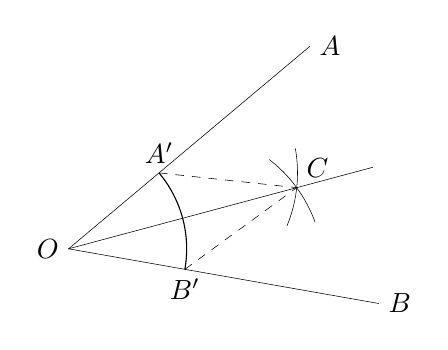
\begin{tikzpicture}[>=stealth,scale=1]
  \tkzSetUpPoint[fill=black]
  % \useasboundingbox(-1,-0.75)rectangle(3.7,1.4);
  \tkzDefPoint(0,0){O}
  \tkzDefPoint(40:4){A}
  \tkzDefPoint(-10:4){B}
  \tkzDefPoint(15:4){C'}
  \tkzDefPoint(40:1.5){A'}
  \tkzDefPoint(-10:1.5){B'}
  \draw(A') arc (40:-10:1.5);
  \tkzDefPoint(15:3){C}
  \tkzDrawSegments(O,A O,B O,C')
  \tkzLabelPoints[right](A,B)
  \tkzLabelPoints[above](A')
  \tkzLabelPoints[below](B')
  \tkzDrawSegments[dashed](A',C B',C)
  \tkzLabelPoints[left](O)
  \tkzCompass[color=black](A',C)
  \tkzCompass[color=black](B',C)
  \tkzLabelPoints[above right](C)
\end{tikzpicture}
\end{document}